\documentclass[12pt, oneside]{article}     
\usepackage[margin=1in]{geometry}                  	
\geometry{letterpaper}                   	
\usepackage{graphicx}				
\usepackage{amssymb}
\usepackage{amsmath}                                                                                                                                                                                                                                                                                                                                                                                                                                                                                                                                                                                          
\usepackage{bm}
\usepackage{float}
\usepackage[nodisplayskipstretch]{setspace}
\setstretch{1.5}
\usepackage{enumitem}

\newif\ifanswers
\answerstrue % comment out to hide answers

\usepackage{fancyheadings}
\pagestyle{fancy}
\lhead {Bayesian Modeling for Socio-Environmental Data }
\rhead{August 1-10, 2016}
\title{Commonly Encountered Problems in Analysis}
\date{August 4, 2016}							


\begin{document}
\maketitle
\thispagestyle{fancy}
\section*{Motivation}
The ability of Bayesian methods to handle hierarchical models in an unusually tidy way is why they are becoming the first choice for complex problems in ecology and conservation biology, problems with multiple unknowns, sources of data and sources of uncertainty. Recall that the posterior distribution of all of the unobserved quantities is proportionate to the joint distributions of the unobserved quantities and the data: 

$$\left[\bm{\theta}\vert\mathbf{y}\right]\propto\underbrace{[\bm{\theta},\mathbf{y}]}_{\text{Factor into sensible parts.}}$$

The starting point for developing hierarchical models is to write a properly factored expression for the proportionality between the posterior and joint distribution of the observed and unobserved quantities. Properly means that the expression for the factored joint distribution obeys the chain rule of probability after assumptions about independence have been made. Bayesian networks, also called directed acyclic graphs, offer a way to visually assure that your model does so.This will be true if there is one unknown and one data set or one hundred unknowns and ten data sets. This factored expression is all that is required to specify a �roll-your-own� MCMC algorithm or to write code in one of the current software packages that sample from the marginal posterior distributions, JAGS, STAN, OpenBUGS etc. The expression for posterior and joint is where you start discussions with statistical colleagues. It should be included in all papers and proposals using Bayesian methods because it communicates virtually everything about where your inferences come from. 

It follows that learning to write proper mathematical and statistical expressions for Bayesian models is 90 percent of the battle. In this exercise, we practice that vital skill. The problems increase in difficulty as we proceed, so it will be important to understand what you did right and wrong before you proceed to the next problem. In addition to practice drawing Bayesian networks and writing posterior and joint distributions, the problems will challenge you to 

1) Choose distributions appropriate for the support of the random variable.

2) Deftly use moment matching to convert means and standard deviations to parameters of distributions.

3) Make inferences on derived quantities.

\section*{Problems}
\begin{enumerate}[leftmargin=*]

\item You are interested in modeling the relationship between per capita income and an index of air pollution for 80 nations around the world (i.e., the Kuznets effect). You hypothesize that air pollution increases then declines as per capita income increases. You have data on the mean (and the standard deviation of the mean) for each country's air quality index (a continuous non-negative variable). The predictor variable (income) is not measured perfectly because it is based on a sample -- you have a mean and a standard deviation of the mean for the per capita income of each county. How would you analyze these data?

\ifanswers
\newpage
\begin{figure}[H]
\center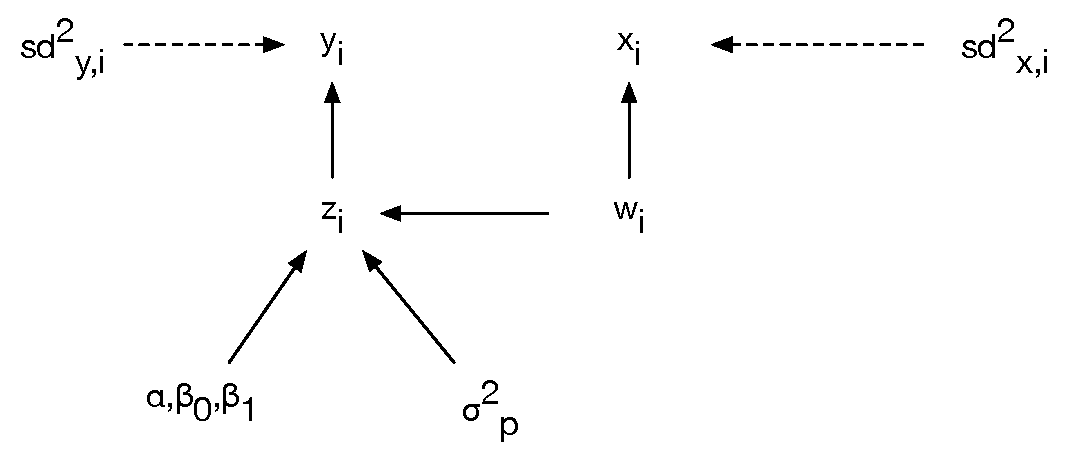
\includegraphics[width=4.75in]{KuznetsDAG.pdf}
\caption{In this DAG, $y_{i}$ and $sd_{y,i}$ and $x_{i}$ and $sd_{x,i}$ and  are the means (and standard deviations of the means) of air quality and per capita income in the $i_{th}$ county.}
\end{figure}
\begin{align*}
\big[ \bm{z}, \bm{w}, \alpha, \bm{\beta}, \sigma^{2}_{p} \mid \bm{y}, \bm{x} \big] \varpropto & \prod^{n}_{i=1} \big[z_{i} \mid g\big( \alpha, \bm{\beta}, w_{i} \big), \sigma^{2}_{p} \big] \big[x_{i} \mid w_{i}, sd^{2}_{x,i} \big] \big[y_{i} \mid z_{i}, sd^{2}_{y,i} \big] \\
& \times \big[z_{i} \big] \big[ w_{i} \big] \big[ \alpha \big] \big[ \beta_{0} \big] \big[ \beta_{1} \big] \big[ \sigma^{2}_{p} \big] 
\end{align*}
\begin{equation*}
\begin{aligned}[c]
&g\big( \alpha, \bm{\beta}, w_{i} \big)\big) = e^{\alpha + \beta_{1}w_{i} + \beta_{2}w_{i}^{2}}\\
&z_{i} \sim \textrm{lognormal}\big(\textrm{log}\big(g\big( \alpha, \bm{\beta}, w_{i} \big)\big), \sigma^{2}_{p} \big) \\
&y_{i} \sim \textrm{lognormal} \big(\textrm{log}\big(z_{i}\big), sd^{2}_{y,i} \big) \\
&x_{i} \sim \textrm{lognormal} \big(\textrm{log}\big(w_{i}\big), sd^{2}_{x,i} \big) \\
&w_{i} \sim \textrm{gamma} \big(.001, .001) \\
\end{aligned}\quad\quad\quad
\begin{aligned}[c]
&z_{i} \sim \textrm{gamma} \big(.001, .001) \\
&\alpha \sim \textrm{normal} \big(0, .001) \\
&\beta_{1} \sim \textrm{normal} \big(0, .001) \\
&\beta_{2} \sim \textrm{normal} \big(0, .001) \\
&\sigma_{p} \sim \textrm{uniform} \big(0, 10)
\end{aligned}
\end{equation*}
\newpage
\fi

\item You have data on the relationship between incidence of lung cancer in households (1 if cancer is present and 0 if no cancer) and radon levels in the house for 1000 houses within 40 counties within a state. You also have data on the clay soil content at the county level, which you heroically assume is know without error. How would you model the effect of radon and soil type on the probability on the probability of lung cancer?

\ifanswers
\newpage
\begin{figure}[H]
\center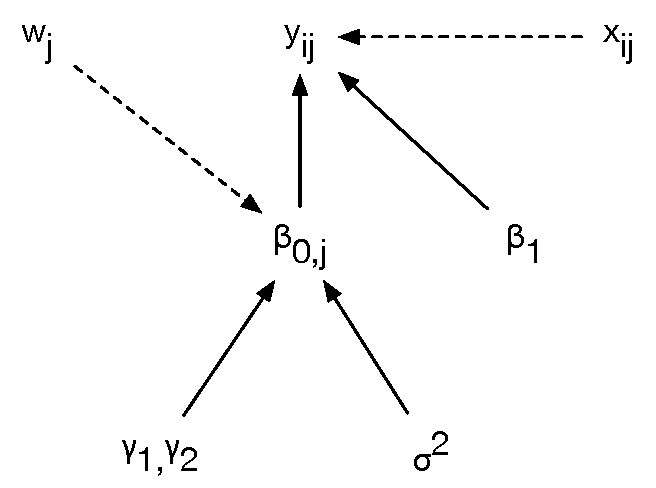
\includegraphics[width=2.75in]{RadonDAG.pdf}
\caption{In this DAG, $x_{ij}$ is the radon level and $y_{ij}$ is an indicator which equals 1 if cancer is present and 0 if it is not in the $i_{th}$ house in the $j_{th}$ county, and $w_{j}$ is the clay soil content in the  $j_{th}$ county.}
\end{figure}
\begin{align*}
\big[\bm{\gamma}, \bm{\beta}, \sigma^{2} \mid \bm{y} \big] \varpropto \prod_{i=1}^{M_{j}} \prod_{j=1}^{N} \big[y_{ij} \mid g\big(\bm{\beta}, x_{ij} \big)\big]  \big[\beta_{0,ij} \mid h\big(\bm{\gamma}, w_{j} \big), \sigma^{2}\big]  \big[\bm{\gamma}\big] \big[\beta_{1}\big] \big[\sigma^{2}\big] 
\end{align*}
\begin{equation*}
\begin{aligned}[c]
&g\big(\bm{\beta}, x_{ij} \big) = \frac{e^{\beta_{0,ij} + \beta_1 x_{ij}}}{1 + e^{\beta_{0,ij} + \beta_1 x_{ij}}} \\
&h\big(\bm{\gamma}, w_{j} \big) = \gamma_{0} + \gamma_{1} w_{j} & \\
&y_{ij} \sim \textrm{Bernoulli} \big(g\big(\bm{\beta}, x_{ij} \big)\big) \\
&\beta_{0} \sim \textrm{normal} \big(h\big(\bm{\gamma}, w_{j} \big), \sigma^{2}) \\
&\beta_{1} \sim \textrm{normal} \big(0, .001) \\
\end{aligned}\quad\quad\quad
\begin{aligned}[c]
&\gamma_{0} \sim \textrm{normal} \big(0, .001) \\
&\gamma_{1} \sim \textrm{normal} \big(0, .001) \\
&\sigma \sim \textrm{uniform} \big(0, 100) \\
& \\
& \\
\end{aligned}
\end{equation*}
\newpage
\fi

\item You have plot level data on diversity of plant communities. The data consist of counts $y_{ij}$ of the number of individuals of species $i$ on $j = 1...J$ same-sized plots, and the total number of individuals on plot $j$ is reported as $n_{j}$. How would you estimate an index $(H)$ of species diversity across the community, where $H=-\sum^{R}_{i=1}p_{i}\textrm{ln}\big(p_{i}\big)$, $(p_{i})$  is the mean proportion of the $i_{th}$ species in in the community, and R is the total number of species present? All estimates must include proper accounting for uncertainty. 

\ifanswers
\newpage
\begin{figure}[H]
\begin{center}
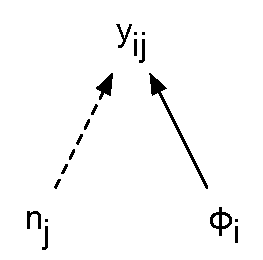
\includegraphics[width=1.5in]{DiversityDAG.pdf}
\caption{In this DAG, $y_{ij}$ is the number of individuals in the $i_{th}$ species observed in the $j_{th}$ plot while $n_{j}$ is the total number of individuals across all species observed in the $j_{th}$ plot.}
\end{center}
\end{figure}
\begin{align*}
\big[\bm{\phi} \mid \mathbf{Y}, \bm{n} \big] \varpropto \prod_{j=1}^{J} \big[\bm{y}_{j} \mid n_{j}, \bm{\phi} \big] \big[\bm{\phi}\big]
\end{align*}
\begin{equation*}
\begin{aligned}[c]
& H = -\sum^{R}_{i=1}\phi_{i}\textrm{ln}\big(\phi_{i}\big) \\
&\bm{y}_{j} \sim \textrm{multinomial}\big(n_{j}, \bm{\phi}\big) \\
&\bm{\phi} \sim \textrm{Dirichlet}\underbrace{\big(1,1,\cdots,1\big)'}_\text{a vector of length R}
\end{aligned}
\end{equation*}

\vspace{10 mm}

where $R$ is the the total number of species across all plots (this comes from the data).
\newpage
\fi

\item You have data on the number of willow seedings that establish on 100 different 10 $\times$ 10 meter plots. Assume these data are measured perfectly, i.e. you did not over or under count seedlings. You also have 5 measurements of soil water and 1 measurement of percent cover (estimated visually) on each plot.  How would you model the effect of soil water and percent bare soil on the number of plants established? You also have paired data of visually estimated cover and actual cover on 15 calibration plots (separate from the 100 plots with seedling and soil water data), where the actual proportion of vegetated soil was laboriously measured using 1 $\times$ 1 meter gridded quadrats.  How would you incorporate uncertainty in the percent cover and soil water covariates in your analysis?

\item Now presume that the 100 plots are arranged in 5 different stream reaches.  You have data on peak runoff in each of the reaches, which you may assume is measured perfectly. You want to understand variation at the catchment scale created by peak runoff.  How would you include these data in the model you developed in problem 4?

\ifanswers
\newpage
\begin{figure}[H]
\begin{center}
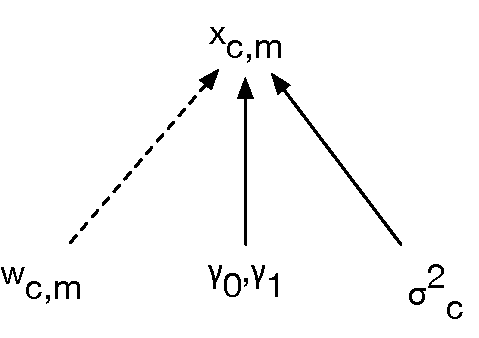
\includegraphics[width=2.5in]{WillowCalibrationDAG.pdf}
\caption{In this DAG, $x_{c,m}$ is the percent cover estimated visually and $w_{c,m}$ is the actual percent cover measured with a quadrat in the $m_{th}$ calibration plot.}
\end{center}
\end{figure}
\begin{align*}
\big[\bm{\gamma}, \sigma^{2}_{c} \mid \bm{x_{c}} \big] \varpropto & \prod_{m=1}^{15} \big[\bm{x}_{c,m} \mid \mu_{m}, \sigma^{2}_{c} \big]  \big[\gamma_{0} \big] \big[\gamma_{1} \big] \big[\sigma^{2}_{c} \big] \\
\end{align*}
\begin{equation*}
\begin{aligned}[c]
&\mu_{m}= \frac{e^{\gamma_{0} + \gamma_1 w_{c,m}}}{1 + e^{\gamma_{0} + \gamma_1 w_{c,m}}} \\
&\alpha_{m} =  \frac{\mu_{m}^{2} - \mu_{m}^{3} - \mu_{m}\sigma^{2}_{c}}{\sigma^{2}_{c}} \\
&\beta_{m} =  \frac{\mu_{m}^{2} - 2\mu_{m}^{2} + \mu_{m}^{3} - \sigma^{2}_{c} + \mu_{m}\sigma^{2}_{c}}{\sigma^{2}_{c}} \\
& x_{c,m} \sim \textrm{beta}\big(\alpha_{m}, \beta_{m}\big) \\
\end{aligned} \quad\quad\quad
\begin{aligned}[c]
&\gamma_{0} \sim \textrm{normal} \big(0, .001) \\
&\gamma_{1} \sim \textrm{normal} \big(0, .001) \\
&\sigma_{c} \sim \textrm{uniform} \big(0, 100) \\
& \\
& \\
\end{aligned}
\end{equation*}

\vspace{10 mm}

To use informed priors on $\gamma_{0}$, $\gamma_{1}$, and $\sigma^{2}_{c}$ we take the mean and standard deviation of each of their MCMC chains. For $\bm{\gamma}$ we must convert the standard deviations to precisions, and for $\sigma^{2}_{c}$ we must moment match to the parameters of a probability distribution whose support is all positive, such as gamma or lognormal. Please see the appendix for details.
\newpage


\begin{figure}[H]
\begin{center}
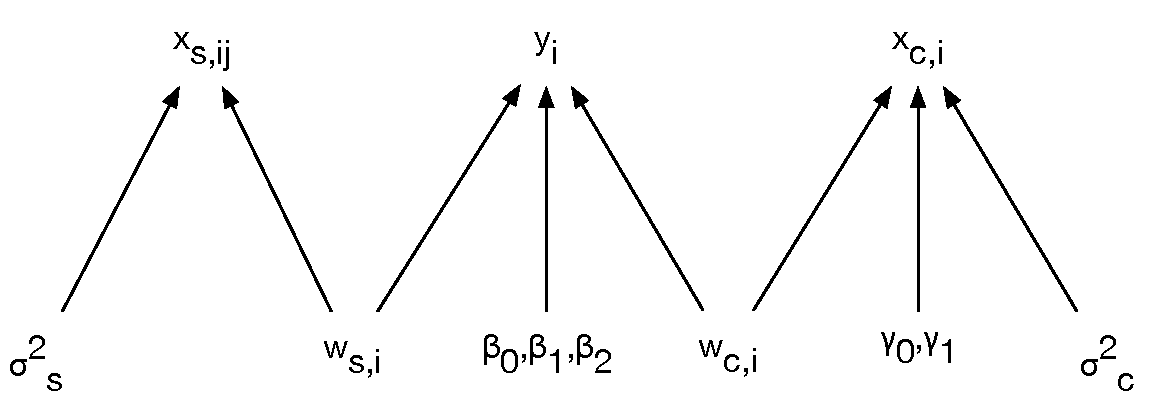
\includegraphics[width=5.75in]{WillowDAG.pdf}
\caption{In this DAG, $y_{i}$ is the number of willow seedlings, $x_{s,ij}$ is the $j_{th}$ measurement of soil water content, and $x_{c,i}$ is a visual estimate of percent cover on the $i_{th}$ plot.}
\end{center}
\end{figure}
\begin{align*}
\big[\bm{\beta}, \bm{\gamma}, \bm{w_{s}}, \bm{w_{c}}, \sigma^{2}_{s}, \sigma^{2}_{c} \mid \bm{y}, \bm{x_{s}}, \bm{x_{c}} \big] \varpropto & \prod_{i=1}^{100} \big[y_{i} \mid g\big(\bm{\beta}, w_{s,i}, w_{c,i}\big)\big] \prod_{j=1}^{5} \big[x_{s,ij} \mid \textrm{log}\big(w_{s,i}\big), \sigma^{2}_{s} \big]\\
&\times  \big[\bm{x}_{c,i} \mid \mu_{i}, \sigma^{2}_{c} \big] \big[\beta_{0} \big] \big[\beta_{1} \big] \big[\gamma_{0} \big] \big[\gamma_{1} \big] \big[w_{s,i}\big] \big[w_{c,i}\big] \big[\sigma^{2}_{s}\big] \big[\sigma^{2}_{c}\big]       
\end{align*}
\begin{equation*}
\begin{aligned}[c]
&g\big(\bm{\beta}, w_{s,i}, w_{c,i} \big) =e^{\beta_{0} + \beta_{1} w_{s,i} + \beta_{2} w_{c,i}}\\
&\mu_{i}= \frac{e^{\gamma_{0} + \gamma_1 w_{c,i}}}{1 + e^{\gamma_{0} + \gamma_1 w_{c,i}}} \\
&\alpha_{i} =  \frac{\mu_{i}^{2} - \mu_{i}^{3} - \mu_{i}\sigma^{2}_{c}}{\sigma^{2}_{c}} \\
&\beta_{i} =  \frac{\mu_{i}^{2} - 2\mu_{i}^{2} + \mu_{i}^{3} - \sigma^{2}_{c} + \mu_{i}\sigma^{2}_{c}}{\sigma^{2}_{c}} \\
&y_{i} \sim \textrm{Poisson} \big(g\big(\bm{\beta}, w_{s,i}, w_{c,i}\big)\big) \\
&x_{s,ij} \sim \textrm{lognormal} \big(\textrm{log}\big(w_{s,i}\big), \sigma^{2}_{s}\big) \\
& x_{c,i} \sim \textrm{beta}\big(\alpha_{i}, \beta_{i}\big) \\
\end{aligned}\quad\quad\quad
\begin{aligned}[c]
&\beta_{0} \sim \textrm{normal} \big(0, .001) \\
&\beta_{1} \sim \textrm{normal} \big(0, .001) \\
&w_{s,i} \sim \textrm{gamma} \big(.001, .001) \\
&w_{c,i} \sim \textrm{uniform} \big(0, 1) \\
&\gamma_{0} \sim \textrm{normal} \big( \gamma_{0,mean}, \gamma_{0,prec}) \\
&\gamma_{1} \sim \textrm{normal} \big( \gamma_{1,mean}, \gamma_{1,prec}) \\
&\sigma_{s} \sim \textrm{uniform} \big(0, 100) \\
&\sigma^{2}_{c} \sim \textrm{gamma} \big(\sigma^{2}_{c,\alpha},\sigma^{2}_{c,\beta}\big)\\
\end{aligned}
\end{equation*}

\vspace{10 mm}
See appendix to understand how we determined the numerical priors on $\gamma_{0}$, $\gamma_{1}$, and $\sigma^{2}_{c}$.


\begin{figure}[H]
\begin{center}
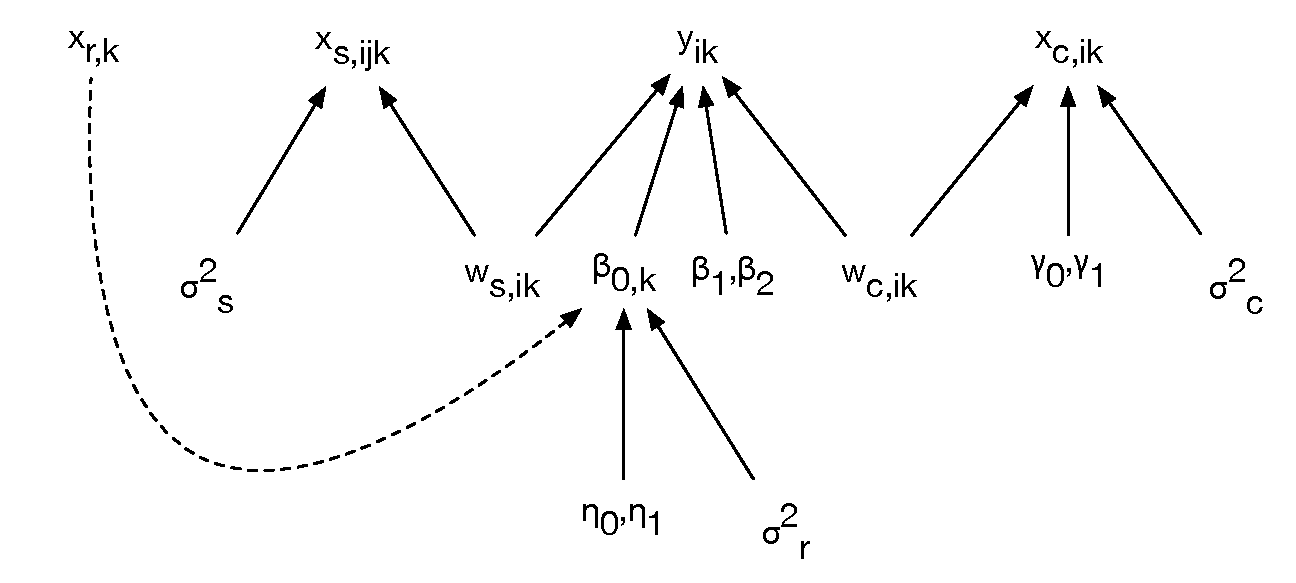
\includegraphics[width=5.5in]{WillowMultiLevelDAG.pdf}
\caption{In this DAG, $y_{ik}$ is the number of willow seedlings, $x_{s,ijk}$ is the $j_{th}$ measurement of soil water content, $x_{c,ik}$ is a visual estimate of percent cover, and $x_{r,k}$ is peak runoff on the $i_{th}$ plot in the $k_{th}$ stream reach.}
\end{center}
\end{figure}
\begin{align*}
\big[\bm{\beta}, \bm{\gamma}, \bm{\eta}, \bm{w_{s}}, \bm{w_{c}}, \sigma^{2}_{s}, \sigma^{2}_{c}, \sigma^{2}_{r} & \mid \bm{y}, \bm{x_{s}}, \bm{x_{c}},  \bm{x_{r}} \big] \varpropto \\
& \prod_{i=1}^{20} \prod_{k=1}^{5} \big[y_{ik} \mid g\big(\bm{\beta}, w_{s,ik}, w_{c,ik}\big)\big]  \big[\beta_{0,k} \mid h\big(\bm{\eta}, x_{r,k}\big)\big] \\
& \times \prod_{j=1}^{5} \big[x_{s,ijk} \mid \textrm{log}\big(w_{s,ik}\big), \sigma^{2}_{s} \big] \big[\bm{x}_{c,ik} \mid \mu_{ik}, \sigma^{2}_{c} \big] \\
& \times \big[\beta_{1} \big] \big[\gamma_{0} \big] \big[\gamma_{1} \big] \big[\eta_{0} \big] \big[\eta_{1} \big]
\big[w_{s,ik}\big] \big[w_{c,ik}\big] \big[\sigma^{2}_{s}\big] \big[\sigma^{2}_{c}\big] \big[\sigma^{2}_{r}\big]         
\end{align*}
\begin{equation*}
\begin{aligned}[c]
&g\big(\bm{\beta}, w_{s,ik}, w_{c,i} \big) =e^{\beta_{0,k} + \beta_{1} w_{s,ik} + \beta_{2} w_{c,ik}}\\
&h\big(\bm{\eta}, x_{r,k} \big) =\eta_{0} + \eta_{1} x_{r,k}\\
&\mu_{ik}= \frac{e^{\gamma_{0} + \gamma_1 w_{c,ik}}}{1 + e^{\gamma_{0} + \gamma_1 w_{c,ik}}} \\
&\alpha_{ik} =  \frac{\mu_{ik}^{2} - \mu_{ik}^{3} - \mu_{ik}\sigma^{2}_{c}}{\sigma^{2}_{c}} \\
&\beta_{ik} =  \frac{\mu_{ik}^{2} - 2\mu_{ik}^{2} + \mu_{ik}^{3} - \sigma^{2}_{c} + \mu_{i}\sigma^{2}_{c}}{\sigma^{2}_{c}} \\
&y_{ik} \sim \textrm{Poisson} \big(g\big(\bm{\beta}, w_{s,ik}, w_{c,ik}\big)\big) \\
&\beta_{0,k} \sim \textrm{normal} \big(h\big(\bm{\eta}, x_{r,k}\big), \sigma^{2}_{r} \big) \\
&x_{s,ijk} \sim \textrm{lognormal} \big(\textrm{log}\big(w_{s,ik}\big), \sigma^{2}_{s}\big) \\
& x_{c,ik} \sim \textrm{beta}\big(\alpha_{ik}, \beta_{ik}\big) \\
\end{aligned}\quad\quad\quad
\begin{aligned}[c]
&\beta_{1} \sim \textrm{normal} \big(0, .001) \\
&w_{s,ik} \sim \textrm{gamma} \big(.001, .001) \\
&w_{c,ik} \sim \textrm{uniform} \big(0, 1) \\
&\eta_{0} \sim \textrm{normal} \big(0, .001) \\
&\eta_{1} \sim \textrm{normal} \big(0, .001) \\
&\gamma_{0} \sim \textrm{normal} \big( \gamma_{0,mean}, \gamma_{0,prec}) \\
&\gamma_{1} \sim \textrm{normal} \big( \gamma_{1,mean}, \gamma_{1,prec}) \\
&\sigma_{s} \sim \textrm{uniform} \big(0, 100) \\
&\sigma^{2}_{c} \sim \textrm{gamma} \big(\sigma^{2}_{c,\alpha},\sigma^{2}_{c,\beta}\big)\\
&\sigma_{r} \sim \textrm{uniform} \big(0, 100) \\
\end{aligned}
\end{equation*}

\vspace{10 mm}
See appendix to understand how we determined the numerical priors on $\gamma_{0}$, $\gamma_{1}$, and $\sigma^{2}_{c}$.
\newpage

\subsubsection*{Appendix}

After convergence, select $t=1,2,...,T$ samples from the MCMC chains for $\gamma_{0}$, $\gamma_{1}$,  and $\sigma^{2}_{c}$.

\begin{equation*}
\begin{aligned}[c]
&\theta^{t}_{\gamma_{0},t} \sim \big[\gamma_{0} \mid \bm{x_{c}} \big] \\
&\theta^{t}_{\gamma_{1},t} \sim \big[\gamma_{1} \mid \bm{x_{c}} \big] \\
&\theta^{t}_{\sigma^{2}_{c},t} \sim \big[\sigma^{2}_{c} \mid \bm{x_{c}} \big] \\
\end{aligned}
\end{equation*}

\vspace{5 mm}

Now approximate the means and variances of each of these chains.
\begin{equation*}
\begin{aligned}[c]
& \gamma_{0,mean} = \frac{1}{T}\sum^{T}_{t=1}\theta^{t}_{\gamma_{0}} \approx \textrm{E}\big[\theta^{t}_{\gamma_{0}} \big]\\
& \gamma_{1,mean} = \frac{1}{T}\sum^{T}_{t=1}\theta^{t}_{\gamma_{1}} \approx \textrm{E}\big[\theta^{t}_{\gamma_{1}} \big]\\
& \sigma^{2}_{c,mean} = \frac{1}{T}\sum^{T}_{t=1}\theta^{t}_{\sigma^{2}_{c}} \approx \textrm{E}\big[\theta^{t}_{\sigma^{2}_{c}} \big]\\
\end{aligned}\quad\quad\quad
\begin{aligned}[c]
& \gamma_{0,var} = \frac{1}{T}\sum^{T}_{t=1}\big(\theta^{t}_{\gamma_{0}}-\gamma_{0,mean}\big)^{2} \approx \textrm{E}\big[\big(\theta^{t}_{\gamma_{0}}- \textrm{E}\big[\theta^{t}_{\gamma_{0}} \big]\big)^{2}\big]\\
& \gamma_{1,var} = \frac{1}{T}\sum^{T}_{t=1}\big(\theta^{t}_{\gamma_{1}}-\gamma_{1,mean}\big)^{2} \approx \textrm{E}\big[\big(\theta^{t}_{\gamma_{1}}- \textrm{E}\big[\theta^{t}_{\gamma_{1}} \big]\big)^{2}\big]\\
& \sigma^{2}_{c,var} = \frac{1}{T}\sum^{T}_{t=1}\big(\theta^{t}_{\sigma^{2}_{c}}-\sigma^{2}_{c,mean}\big)^{2} \approx \textrm{E}\big[\big(\theta^{t}_{\sigma^{2}_{c}}- \textrm{E}\big[\theta^{t}_{\sigma^{2}_{c}} \big]\big)^{2}\big]\\
\end{aligned}
\end{equation*}

\vspace{5 mm}

Lastly, for $\gamma_{0}$ and $\gamma_{1}$ convert the standard deviations to precisions, and for $\sigma^{2}_{c}$ we moment match to the $\alpha$ and $\beta$ parameters in a gamma distribution.

\begin{equation*}
\begin{aligned}[c]
& \gamma_{0,prec} = \frac{1}{\gamma_{0,var}} \\
& \gamma_{1,prec} = \frac{1}{\gamma_{1,var}} \\
\end{aligned}\quad\quad\quad
\begin{aligned}[c]
& \sigma^{2}_{c,\alpha} = \frac{\big(\sigma^{2}_{c,mean}\big)^{2}}{\big(\sigma^{2}_{c,var}\big)^{2}} \\
& \sigma^{2}_{c,\beta} = \frac{\sigma^{2}_{c,mean}}{\big(\sigma^{2}_{c,var}\big)^{2}}
\end{aligned}
\end{equation*}
\fi

\end{enumerate}

\end{document}

